\documentclass{article}
\usepackage{float}
\usepackage{listingsutf8}
\usepackage{graphicx}
\usepackage{appendix}
\usepackage[colorlinks]{hyperref}
\usepackage{amsmath}
\usepackage{indentfirst}
\usepackage{enumerate}
\lstset{frameshape={RYRYNYYYY}{yny}{yny}{RYRYNYYYY}, backgroundcolor=\color[RGB]{245,245,244}}
\title{The Design and Implementation of a Multi-access Threaded Queue}
\author{Xihuai Wang 16337236}
\date{}

\begin{document}
	\maketitle
	\tableofcontents
	\section{Analytics and Design} % (fold)
	\label{sec:analytics}
	To make sure that the queue works well when multiple threads inserting and multiple threads extracting from the queue, the queue should guarantee that all the threads see the same contents at the same time. That is, we should guarantee that access to the last element and pushing new element into the queue will not happen simultaneously, and that access to the first element and poping the head of the queue will not happen simultaneously, as well as that requireing the size or checking whether the queue is empty will not happen when threads are trying to modify the queue. 
	\par To analyse the performance of the queue, we need a comparsion, the same operations in serial case.
	\par My design is that I encapsulates the queue template class from the stardand library and makes it support multi-access. To avoid unnecessarily blocking threads, we need 2 mutexlock, one is used to control the head of the queue, the other is used to control the tail of the queue. Both of the two is used to pretend modification of the queue when requireing the size or checking the status of the queue. Besides, the two methods the template class designed provided, front() and back() will return a copy of the element in the corresponding place rather return a reference to the element, because the threads may make a mess if that.
	\par To analyse the performance, I calculate the time the multi-threads version used to insert and extract to and from the queue a certain times, and the time the serial version used.
	% section analytics (end)

	\section{Implementation Code} % (fold)
	\label{sec:implementation_code}
	The multi-access queue is implemented using pthread library.This section shows the main components of the code.
	\par The declaration of the MultiAccessQueue template class is shown in code block below.
	\begin{lstlisting}[language=c++, numbers=left,	numberstyle=\tiny,basicstyle=\small]
	template<typename T>
	class MultiAccessQueue
	{
	public:
	  MultiAccessQueue();
	  ~MultiAccessQueue();
	  bool empty();
	  size_t size();
	  T front();
	  T back();
	  void push(T ele);
	  void pop();

	private:
	  std::queue<T> oriQue;
	  pthread_mutex_t headLock;
	  pthread_mutex_t tailLock;
	};
	\end{lstlisting}
	\par The queue instantiation and the 2 locks are the most important designs. Most methods of queue are overloaped.
	\par As an example, the implementation of size() and push() methods are shown in the following code block.
	\begin{lstlisting}[language=c++, numbers=left,	numberstyle=\tiny,basicstyle=\small]
	template<typename T>
	size_t MultiAccessQueue<T>::size()
	{
	  pthread_mutex_lock(&headLock);
	  pthread_mutex_lock(&tailLock);
	  size_t ret = oriQue.size();
	  pthread_mutex_unlock(&headLock);
	  pthread_mutex_unlock(&tailLock);
	  return ret;
	}

	template<typename T>
	void MultiAccessQueue<T>::push(T ele)
	{
	  pthread_mutex_lock(&tailLock);
	  oriQue.push(ele);
	  pthread_mutex_unlock(&tailLock);
	}
	\end{lstlisting}
	\par The main work is to lock and unlock the mutex lock.
	\par And the flow chart of the program to use this queue is shown is figure \ref{fig:Multiqueue}.
	\begin{figure}[H]
		\centering
		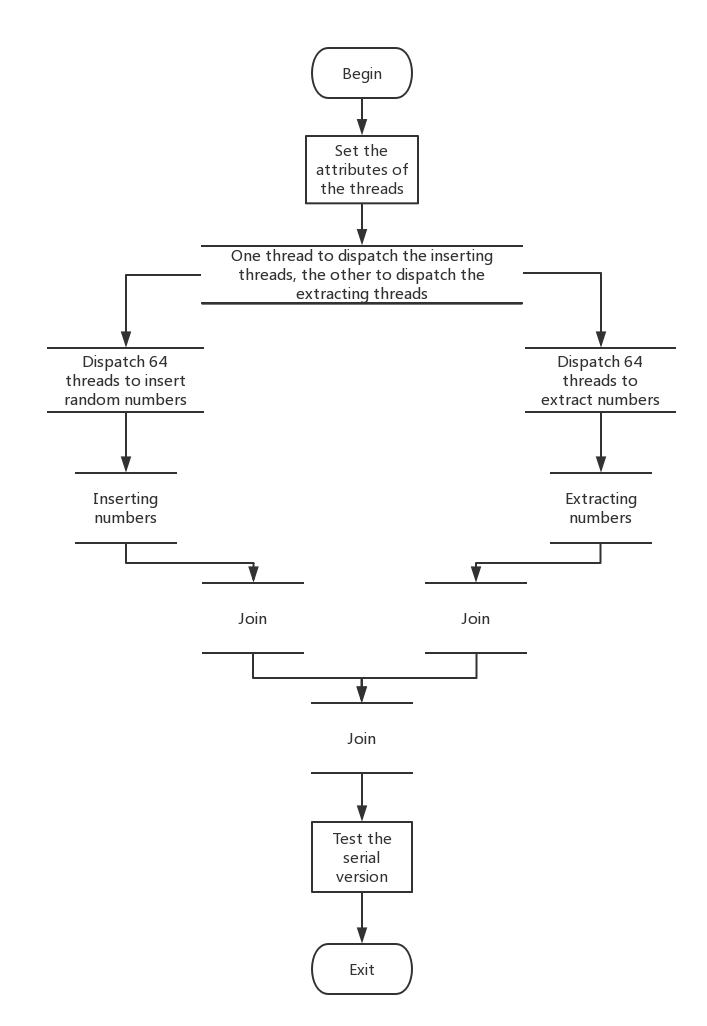
\includegraphics[scale=0.4]{imgs/Multiqueue.png}
		\caption{Flow Chart}
		\label{fig:Multiqueue}
	\end{figure}
	The program here used the fork-join mode, and the tricknesses here are:
	\begin{enumerate}[1.]
		\item The argument pointers passed to the new threads should point to independent memory, otherwise there will be a mess. So I choose the way that "new" a temporary variable $\to$ copy the variable expected to pass $\to$ pass the temporary variable $\to$ delete it in new thread. 
		\item In order to divide a loop to multiple threads, the loop control variables should be initialized differently and cover all the loop range. The method I used here is dividing the loop range into 64 equal parts, except for the last one.
		\item If a thread want to extract a element from the queue, it must wait until the queue is not empty. I use a spin wait here.
	\end{enumerate}
	\par I have also implemented the queue using OpenMP interfaces, and with OpenMp, it is easier to implement the program that uses the queue, but the work to implement the queue itself is not easier, let's show the declaration of the multi-access queue.
	\begin{lstlisting}[language=c++, numbers=left,	numberstyle=\tiny,basicstyle=\small]
	template<typename T>
	class MultiAccessQueue
	{
	public:
	  MultiAccessQueue();
	  ~MultiAccessQueue();
	  bool empty();
	  size_t size();
	  T front();
	  T back();
	  void push(T ele);
	  void pop();

	private:
	  std::queue<T> oriQue;
	  omp_lock_t headLock;
	  omp_lock_t tailLock;
	};
	
	\end{lstlisting}
	And the trunk of the program that uses the queue is shown below.
	\begin{lstlisting}[language=c++, numbers=left,	numberstyle=\tiny,basicstyle=\small]
	omp_set_num_threads(THREADS);
	omp_set_nested(1);
	double start, stop;
	start = omp_get_wtime();
	#pragma omp parallel sections
	{
	    #pragma omp section
		{
	    printf("Totally %d threads\n", omp_get_num_threads());
		}
	    #pragma omp section
		{
		  insert();
		}
	    #pragma omp section
		{
		  extract();
		}
	}
	stop = omp_get_wtime();
	\end{lstlisting}
	Clearly, the implementation is more concise that using pthread.
	% section implementation_code (end)
	\section{Result} % (fold)
	\label{sec:result}
	The results that the programs run in my 4-core, 8-thread computer, are shown in table \ref{tab:ResultParallel} and \ref{tab:ResultSerial}, the times of insertions and extractions vary from 1000 to 100000000.
	\begin{table}[H]
		\begin{minipage}{0.48\linewidth}
			\centering
			\caption{Results of Parallel Version}	
			\begin{tabular}{|l|c|}
			\hline
			Number of operation & Time(s) \\
			\hline 
			1000 & 0.020\\
			10000 & 0.024\\
			100000 & 0.037\\
			1000000 & 0.447\\
			10000000 & 5.350\\
			100000000 & 41.715\\
			\hline
			\end{tabular}
			\label{tab:ResultParallel}
		\end{minipage}
		\begin{minipage}{0.48\linewidth}
			\caption{Results of Serial Version}	
			\begin{tabular}{|l|c|}
			\hline
			Number of operation & Time(s) \\
			\hline 
			1000 & 0.000\\
			10000 & 0.002\\
			100000 & 0.022\\
			1000000 & 0.272\\
			10000000 & 1.453\\
			100000000 & 25.035\\
			\hline
			\end{tabular}
			\label{tab:ResultSerial}
		\end{minipage}
	\end{table}
	
	% section result (end)
	\section{Conclusion} % (fold)
	\label{sec:conclusion}
	Obviously and surprisingly that the parallel version of program is much slower. But the reason is also obvious: 
	\begin{enumerate}[1.]
	\item The parallel spends too much time scheduling the processes, that is because the number of threads is 130 but my computer has only 8 threads at all. 
	\item The task per thread does is easy and low load in comparison. 
	\item The CPU resource is wasted in spin wait, and thus the efficiency is lower.
	\end{enumerate}
	\par By the way, it is even slower when using OpenMp, the reason may be that it is hard to control the critical sections, and the resource is wasted when waiting.
	% section conclusion (end)

\end{document}